\documentclass[../../../All.tex]{subfiles}
%%---------------------------%
%%---- Обычный файл      ----%
%%---------------------------%
%\sloppy
%\documentclass[14pt,a4paper,oneside]{extarticle}	% Размер основного шрифта и формата листа
%\usepackage{xltxtra}						% Используется для вывода логотипа XeLaTeX
%\usepackage{xunicode}						% Кодировка документа
%\usepackage{polyglossia}					% Загружает пакет многоязыковой верстки
%\newfontfamily\russianfont{Book Antiqua}
%%\setmainfont{Liberation Serif}						% Основной шрифт текста
%\setmainfont{Book Antiqua}
%\setdefaultlanguage{russian}				% Основной язык текста
%\setotherlanguage{english}					% Дополнительный язык текста
%\linespread{1}							% Межстрочный интервал выбран полуторным
%\usepackage[left=2.5cm,
%right=1.5cm,vmargin=2.5cm]{geometry} % Отступы по краям листа
%\bibliographystyle{ugost2008}
%
%\usepackage{xcolor}
%\usepackage{hyperref}
%% Цвета для гиперссылок
%\definecolor{linkcolor}{HTML}{359B08} % цвет ссылок
%\definecolor{urlcolor}{HTML}{799B03} % цвет гиперссылок
%\hypersetup{pdfstartview=FitH,  linkcolor=linkcolor,urlcolor=urlcolor, colorlinks=true}
%
%%---------------------------%
%%---- Пакеты расширений ----%
%%---------------------------%
%\usepackage{xcolor}
%\usepackage{hyperref}
%% Цвета для гиперссылок
%\definecolor{linkcolor}{HTML}{359B08} % цвет ссылок
%\definecolor{urlcolor}{HTML}{799B03} % цвет гиперссылок
%\hypersetup{pdfstartview=FitH,  linkcolor=linkcolor,urlcolor=urlcolor, colorlinks=true}
%
%
%\usepackage{verbatim,indentfirst}
%\usepackage{cite,enumerate,float}
%\usepackage{amsmath,amssymb,amsthm,amsfonts}
%
%%---------------------------%
%%--- Вставка иллюстраций ---%
%%---------------------------%
%\usepackage{graphicx}
%\usepackage{subfigure}
%\usepackage{fontspec}
%%\graphicspath{{Images/}}

\begin{document}
%	\pagestyle{empty} %  выключаенм нумерацию
%\setcounter{page}{3}% Нумерация начинается с третьей страницы
%\renewcommand{\contentsname}{\center{Содержание}}
%\tableofcontents


	\section{Импульс силы. Гиря и две нити}


\begin{figure}[H] 	% Окружение для вставки иллюстрации
	\centering 		% Выравнивание по центру
	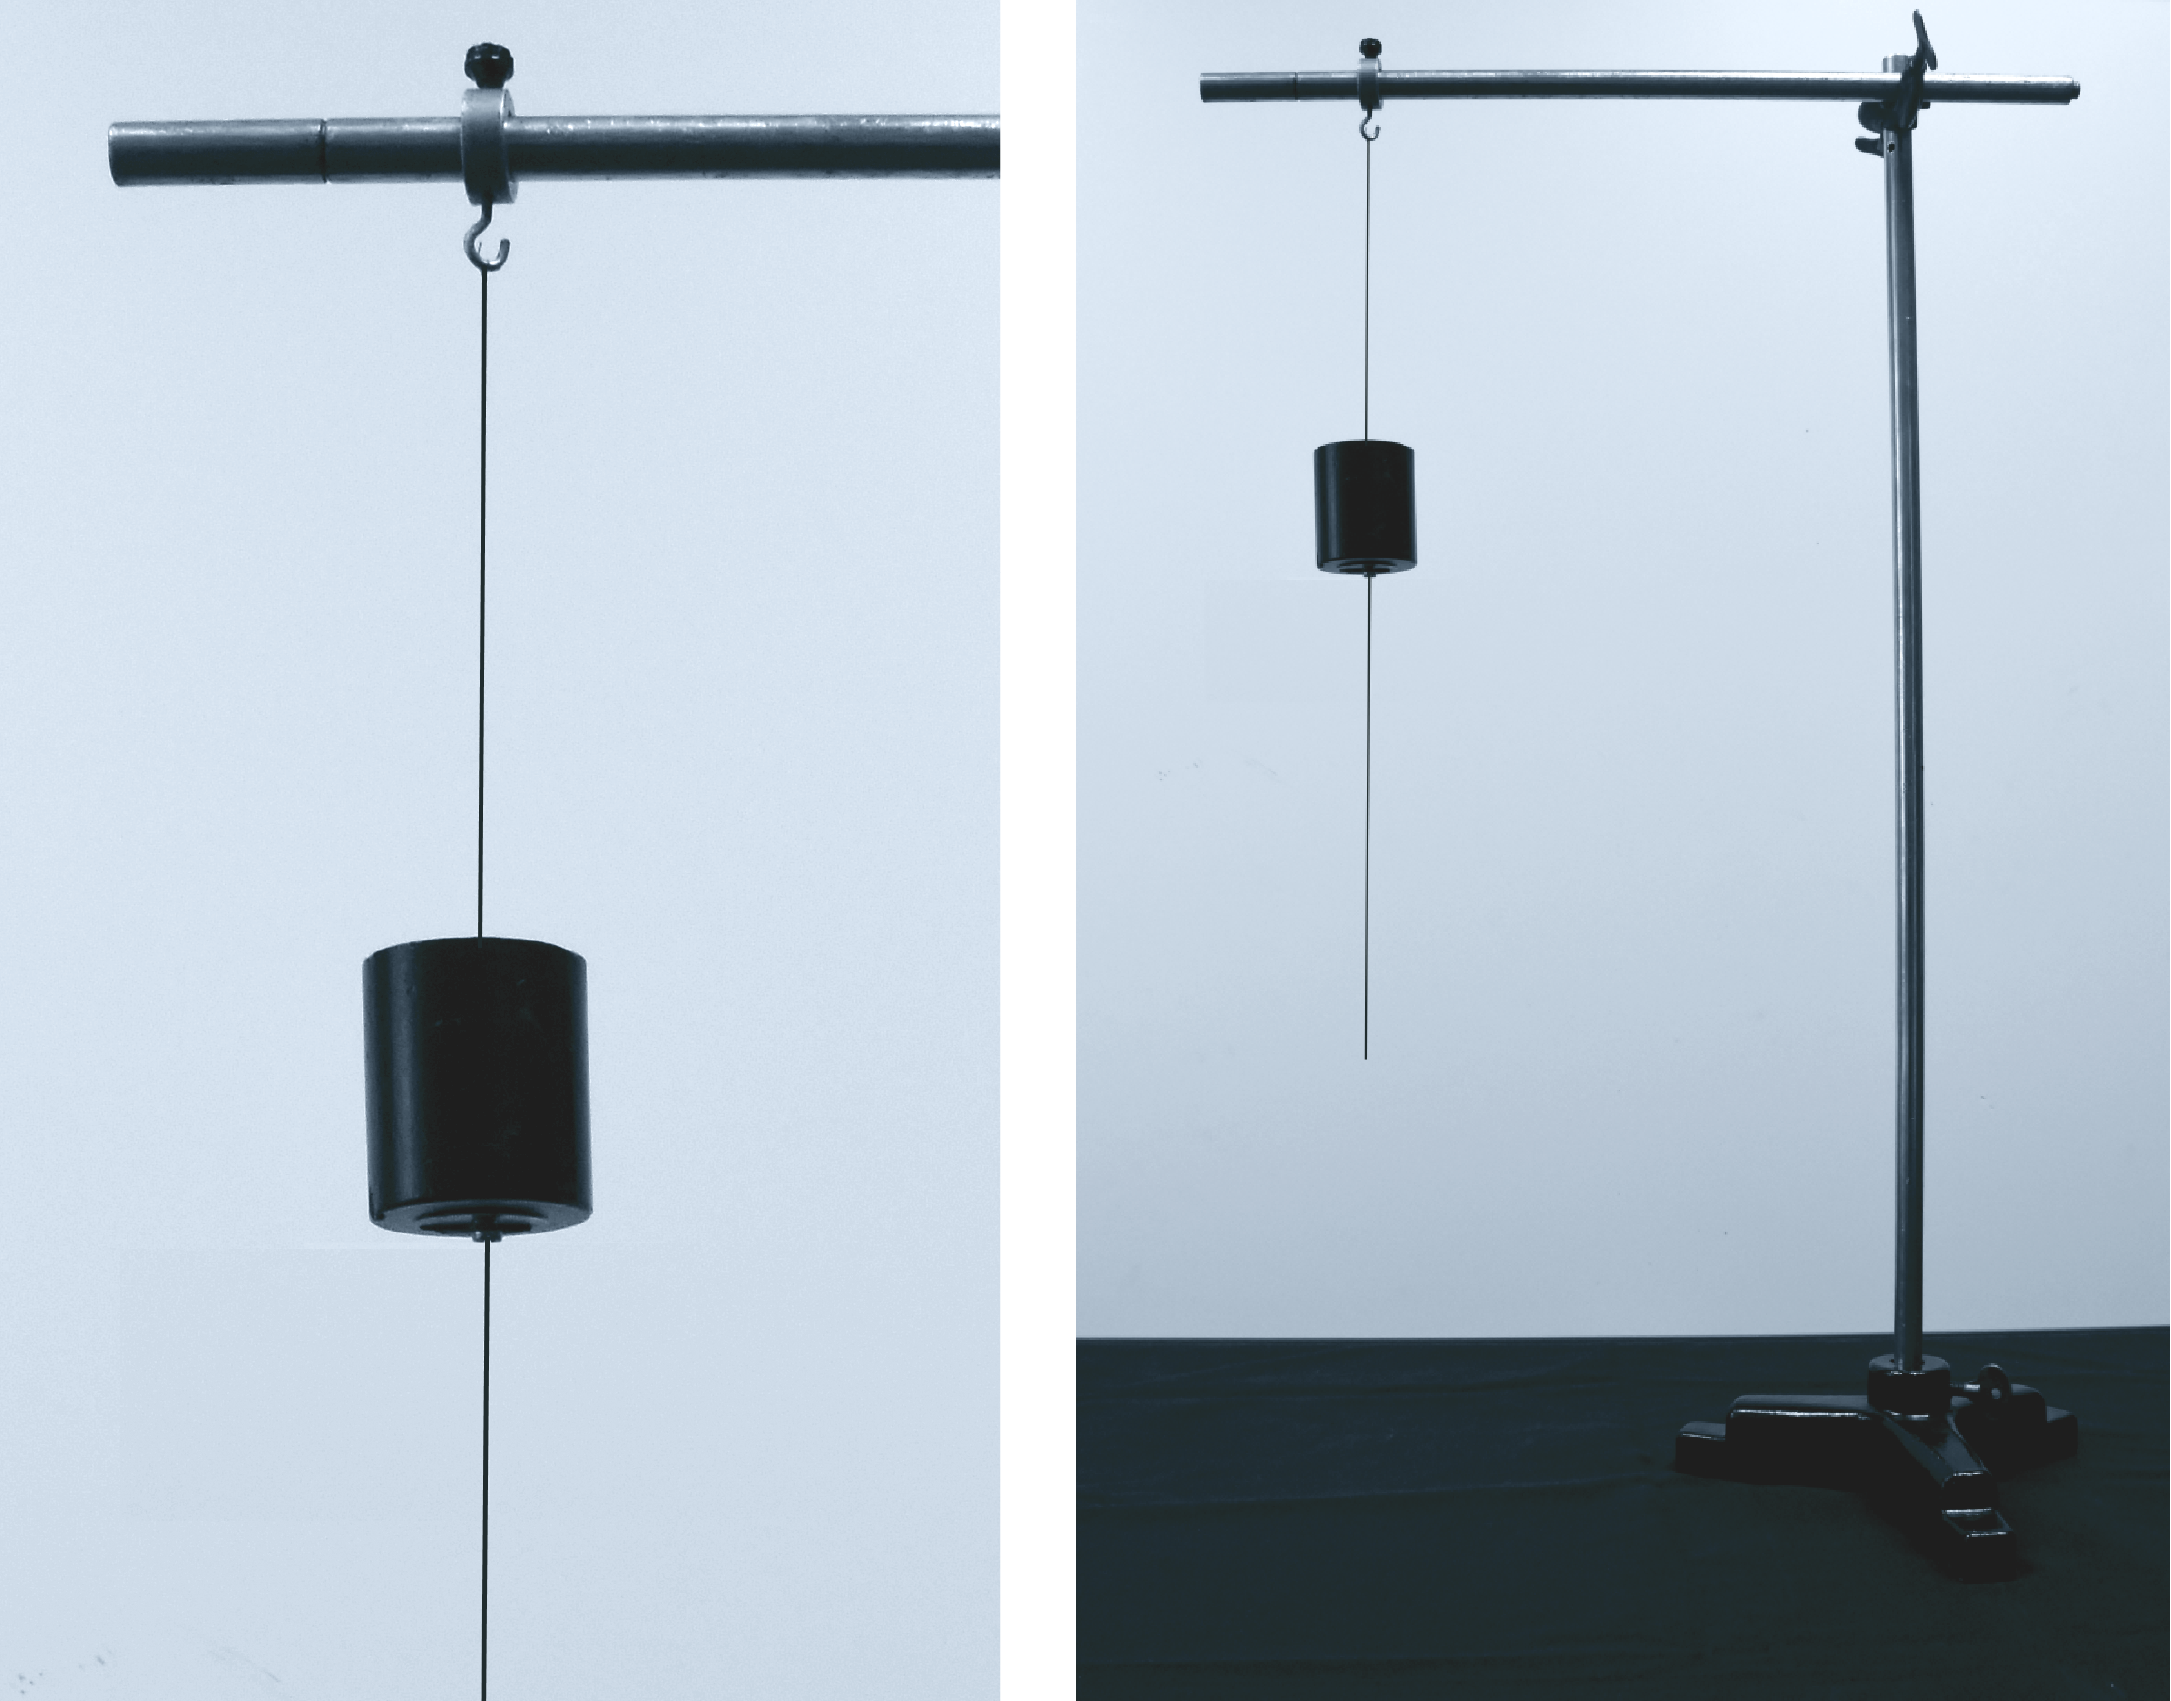
\includegraphics[width=0.7\linewidth]{inertia-2.png}
	\caption{Демонстрация явления инерции}
\end{figure}

\subsection*{\textcolor{PineGreen}{Оборудование}}

\begin{enumerate}
	\item Физический штатив с муфтой и крючком.
	\item Гиря с крючками, ввинченными в верхний и нижний торцы.
	\item Несколько нитей одинаковой толщины и длины.
	\item Резиновый коврик, используемый для амортизации удара.
\end{enumerate}

\subsection*{\textcolor{PineGreen}{Основные определения}}

Величина, количественно определяющая те действия тел друг 
на друга, которые вызывают ускорения, называется силой. 
С одной стороны, сила есть количественная мера действий тел друг на друга.
С другой стороны, сила есть количественная мера тех действий, которые вызывают ускорения.  

Конечная скорость движения тел определяется не только самой 
силой, но и временем действия этой силы. 

Импульсом называется мера механического движения, равная для материальной точки произведению ее массы $ m $ на скорость $ \textbf{v} $.
Такая величина как импульс $ \textbf{p} = m\textbf{v} $ — является векторной, направленной так же, как скорость точки.
Импульс $ \textbf{P} $ механической системы равен геометрической сумме импульсов всех ее точек, или произведению массы $ М $ всей системы на скорость $ \textbf{V}_{c} $ её центра масс: $$ \textbf{P} = \sum m_{i} \textbf{v}_{i} =  M\textbf{V}_{c}. $$

При действии силы \textbf{F} импульс точки изменяется в общем случае и численно и по направлению; это изменение определяется вторым (основным) законом динамики.
Изменение импульса системы происходит под действием только внешних сил, то есть сил, действующих на систему со стороны тел, в эту систему не входящих.

Импульс силы \textbf{S} — это сложная физическая величина, которая 
одновременно учитывает влияние модуля, направления и времени 
действия силы на изменение состояния движения тела.
Импульс силы $\textbf{S} = \textbf{F}\Delta t $ является вектором, по направлению совпадающим с направлением вектора силы \textbf{F}. 
Импульс системы — величина векторная и направлен он в ту же сторону, что и вектор результирующей силы $ \textbf{F}_{p} $.

В новых понятиях второй закон Ньютона можно прочитать следующим образом: 
\begin{flushleft}
	\textit{изменение импульса тела равно импульсу всех сил, действовавших на него:}
\end{flushleft}

\begin{center}
		$\textbf{F}\Delta t = m\textbf{v}_{2} - m\textbf{v}_{1} $ или $\textbf{F}\Delta t = \Delta(m\textbf{v}). $
\end{center}

Именно в таком виде закон был впервые сформулирован самим И. Ньютоном.

\subsection*{\textcolor{PineGreen}{Краткое описание демонстрации}}

К штативу, установленном на ровной поверхности, при помощи тонкой нити подвешивается тело (цилиндр массой $ 200 $ г).
Прочность нитей подбирается так, чтобы верхняя нить могла только удерживать тело, не разрываясь.
В нижнюю часть этого цилиндра ввинчивается крючок с привязанным к нему такой же нитью.
Для амортизации удара на стол кладется резиновый коврик.

Если во время опыта нижнюю нить резко с большой силой дернуть, то она разорвется, а верхняя как бы не «почувствует» сильного рывка (точка 2 на рис.\ref{inertia-3}). 
Причина кроется в том, что большая сила \textbf{F} действует на груз в течение очень короткого времени $ \Delta t $. 
Это время затрачивается только на создание деформации нижней нити во время рывка. 
Тело массой \textit{m} получает незначительный импульс силы, поэтому не успевает набрать скорость и сдвинуться с места.
По этой причине в верхней нити не возникают дополнительных деформации, и она оcтается целой. 

Если нижнюю нить потянуть плавно с небольшой силой, то верхняя нить оборвется (точка 1 на рис.\ref{inertia-3}) и груз упадет.
Это объясняется тем, что действие небольшой силы \textbf{F} за счет продолжительности взаимодействия, т.е. большого $ \Delta t $, приводит к тому, что телу сообщается существенный импульс силы \textbf{F}$ \Delta t $.
За рассматриваемый промежуток времени скорость, а, соотвественно, импульс тела успевают измениться. 
Это приводит к небольшому смещению тела, из-за чего в верхней нити возникает дополнительная деформация.
Благодаря тому, что в опыте используется тонка нить, деформации быстро достигают предела прочности и верхняя нить обрывается. 

\textit{Устройство и применение прибора}. В конструкции штатива муфта обеспечивает устойчивое крепление деталей штатива или других приборов, параллельно или перпендикулярно вертикальной стойке штатива.
Это условие в физическом штативе имеет существенное значение, т.к. приходится, например, закреплять в штативе блок на стержне, динамометры лабораторные и демонстрационные и другие приборы и приспособления.

%Кольцо на одной стороне имеет плоскую форму, что позволяет устанавливать более устойчиво приборы и приспособления с плоскими основаниями.

\subsection*{\textcolor{PineGreen}{Теория}}

В рассматриваемом эксперименте движение гири определяется следующим уравнением (второй закон Ньютона в векторной форме) 
\begin{equation}\label{inertia-eq6}
	\textbf{F}_{\text{н}} + \textbf{F}_{\text{в}} + m\textbf{g} = m\textbf{a},
\end{equation}
где $ \textbf{F}_{\text{н}} $, $ \textbf{F}_{\text{в}} $ — векторы сил натяжения нижней и верхней нитей соответственно, $ m\textbf{g} $ — вектор силы тяжести, $ \textbf{a} $ — ускорение груза.

\begin{figure} 
	\centering 	
	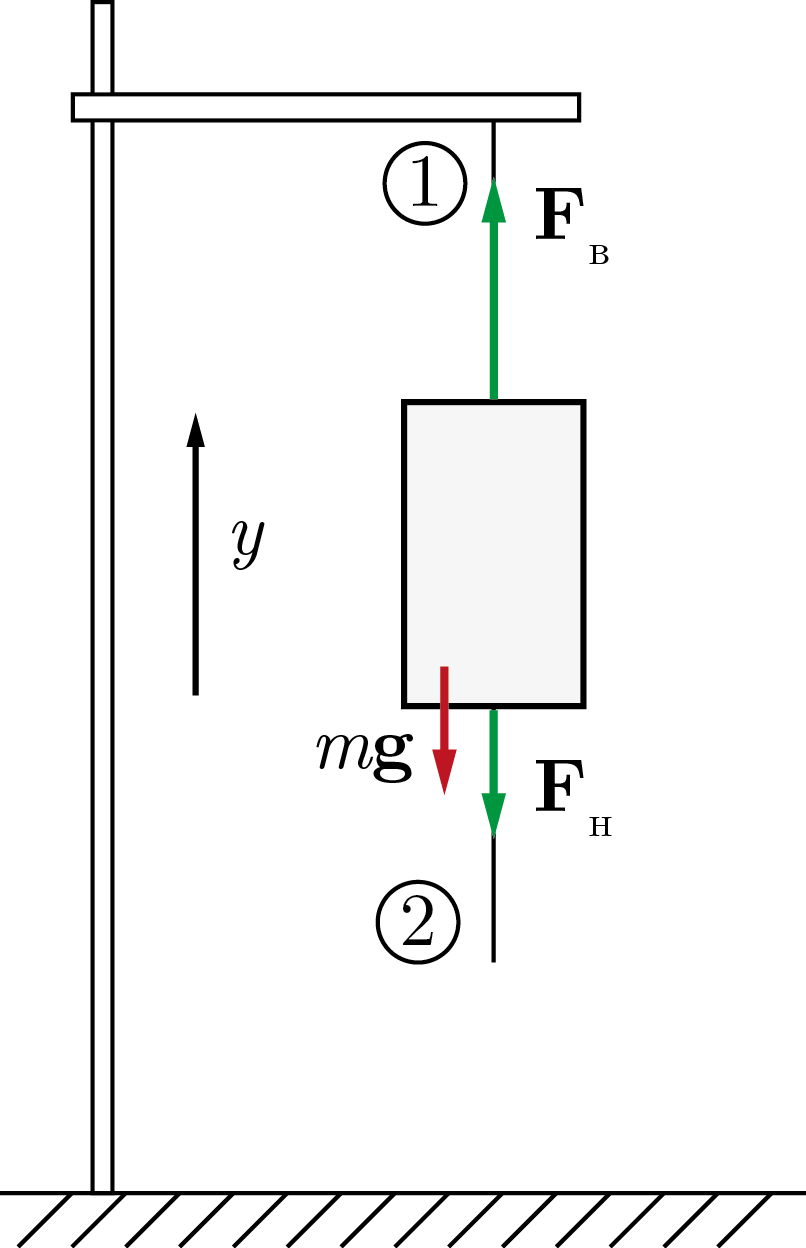
\includegraphics[width=0.3\linewidth]{inertia-3.png}
	\caption{Схематичное изображение подвешенного на нити груза}
	\label{inertia-3}
\end{figure}

При медленном натяжении имеет место «статическое» распределение сил (ускорение мало или $ a \longrightarrow 0$). В проекции на ось $ y $ уравнение [\ref{inertia-eq6}] имеет вид:
\begin{equation}\label{inertia-eq7}
- F_{\text{н}} + F_{\text{в}} - mg = 0,\\
F_{\text{в}} > F_{\text{н}},
\end{equation}
то есть сила натяжения верхней нити превышает силу натяжения со стороны нижней нити на величину $ mg $.

При резком натяжении нити ускорение движения груза будет направлено вниз, проекция уравнения [\ref{inertia-eq6}] имеет вид:
\begin{equation}\label{inertia-eq8}
F_{\text{в}} - F_{\text{н}} -  mg = - ma, \\
F_{\text{н}} = F_{\text{в}} - mg + ma, 
\end{equation}
откуда $F_{\text{н}} > F_{\text{в}}$, поэтому при значительном ускорении $ a $ (резкий рывок) в первую очередь обрывается нижняя нить.

Таким образом, разница в обрыве нижней или верхней нитей обусловливается присутствием в системе тела большой массы, подвешенного за верхнюю нить.
В случае резкого рывка смещение гири в силу ее инертности оказывается малым, поэтому характерное время растяжения верхней нити значительно превышает время растяжения нижней.
Поэтому для нижней нити разрывное натяжение «наступает» раньше.

\end{document}
